\documentclass[twocolumn]{article}
\usepackage{booktabs}
\usepackage{listings}
\usepackage{xcolor}
\usepackage{geometry}
\geometry{margin=1in}
\usepackage{amsmath}
\usepackage{graphicx}
\usepackage{float}
\usepackage{moresize}

\usepackage[backend=biber,style=authoryear]{biblatex} % Choose your style
\addbibresource{references.bib} % Use the name of your .bib file
    

\definecolor{codegray}{gray}{0.9}
\definecolor{deepblue}{rgb}{0,0,0.5}
\definecolor{deepred}{rgb}{0.6,0,0}
\definecolor{deepgreen}{rgb}{0,0.5,0}

\lstdefinestyle{mypython}{
    backgroundcolor=\color{codegray},   
    commentstyle=\color{deepgreen},
    keywordstyle=\color{deepblue},
    numberstyle=\tiny\color{gray},
    stringstyle=\color{deepred},
    basicstyle=\ttfamily\footnotesize,
    breakatwhitespace=false,         
    breaklines=true,                 
    captionpos=b,                    
    keepspaces=true,                 
    numbers=left,                    
    numbersep=5pt,                  
    showspaces=false,                
    showstringspaces=false,
    showtabs=false,                  
    tabsize=4,
    language=Python
}


% Custom author info
\pagenumbering{gobble}
\title{
    \textbf{\small COMS4047A}\\[0.5em]
    \textbf{Reinforcement Learning}\\[1em]
    {\Huge \textbf{Assignment}}\\[3cm]
    
\includegraphics[width=0.4\textwidth]{download.png}
}

\author{
    \small
    \begin{tabular}{l}
    \textbf{Taboka Chloe Dube - 2602515} \\
    \textbf{Wendy Maboa - 2541693} \\
    \textbf{Liam Brady - 2596852} \\
    \textbf{Refiloe Mopeloa - 2333776}
    \end{tabular}
}

\begin{document}

\begin{titlepage}  % <- ensures it's treated as a full separate page
    \maketitle
\end{titlepage}


\newpage

\pagenumbering{arabic} 
\setcounter{page}{1}
\section*{Introduction}
Crafter is a procedurally generated 2D survival game designed as a benchmark for reinforcement learning
 research. It features a diverse set of tasks including resource gathering, tool crafting, creature combat, and
 achievement hunting, all while managing survival mechanics like hunger and health. This report will provide an overview of implementation of agents in Crafter using DQN and PPO algorithms.

\section*{In-class Algorithm: DQN}

\section*{Out-of-class Algorithm: PPO}

PPO (Proximal Policy Optimization) is a reinforcement learning algorithm that trains an agent by optimizing its decision-making policy. It works by collecting data through interactions with an environment and then using a clipped objective function to make stable updates to the policy. This approach is known for being more stable, efficient, and easier to implement than some other policy gradient methods \parencite{schulman}.

\subsection*{Motivation}
PPO (Proximal Policy Optimization) is a good choice for the Crafter environment because it provides a strong balance of stability, sample efficiency, and simplicity while effectively handling the environment's key challenges, such as sparse rewards, long-term reasoning, and procedural generation. 

In addition these are the following theoretical benefits of PPO:
\begin{itemize}
    \item \textbf{Stable Policy Updates:} The Crafter environment is complex and dynamic, where large, unconstrained policy updates could easily destabilize training and cause the agent to forget beneficial behaviors. PPO's clipping mechanism limits how much the policy can change at each step, ensuring stable and controlled learning.
    \item \textbf{Sample Efficiency:} Crafter involves many different achievements and complex interactions, meaning efficient use of experience is crucial. PPO is relatively sample-efficient because it can reuse collected data over multiple training epochs (mini-batches) without significant instability, unlike other on-policy methods that only use data once.
    \item \textbf{Facilitates Exploration:} The PPO objective often includes an entropy bonus term, which encourages the agent to explore different actions and strategies. This is vital in Crafter, which features wide, procedurally generated worlds and independent achievements that require broad exploration to discover all possibilities.
\end{itemize}

\subsection*{Hyperparamters used accross all agents}
\item \textbf{PPO Training:} These hyperparameters were standardized for all agents so as to make sure the comparison is done based on the differing algorithms and not hyperparameter tuning.
\begin{itemize}
    \item Learning rate: $3 \times 10^{-4}$
    \item Rollout steps (n\_steps): 2,048
    \item Batch size: 64
    \item Epochs per update: 10
    \item Discount factor ($\gamma$): 0.99
    \item GAE lambda ($\lambda$): 0.95
    \item Clip range: 0.2
    \item Entropy coefficient: 0.01
\end{itemize}

\subsection*{Baseline Implementation}
The baseline agent was implemented using the Stable-Baselines3 PPO algorithm. The initial hyperparameters were chosen to provide stable learning without aggressive updates, ensuring reproducibility. The agent at this point perceives the environment through single still images (frames) rather than continuous sequences, meaning it has only a limited view of the environment at each step.
\subsubsection*{Observations and Performance}
The baseline PPO agent exhibited some exploratory behavior and moderate learning progress. However, its limited temporal awareness significantly constrained performance. The average episodic reward stabilized around \textbf{3.26}, with the maximum reward achieved being \textbf{7.1}.
The following figures show the reward and survival distribution rates over 100 episodes:
\begin{figure}[H]
    \centering
    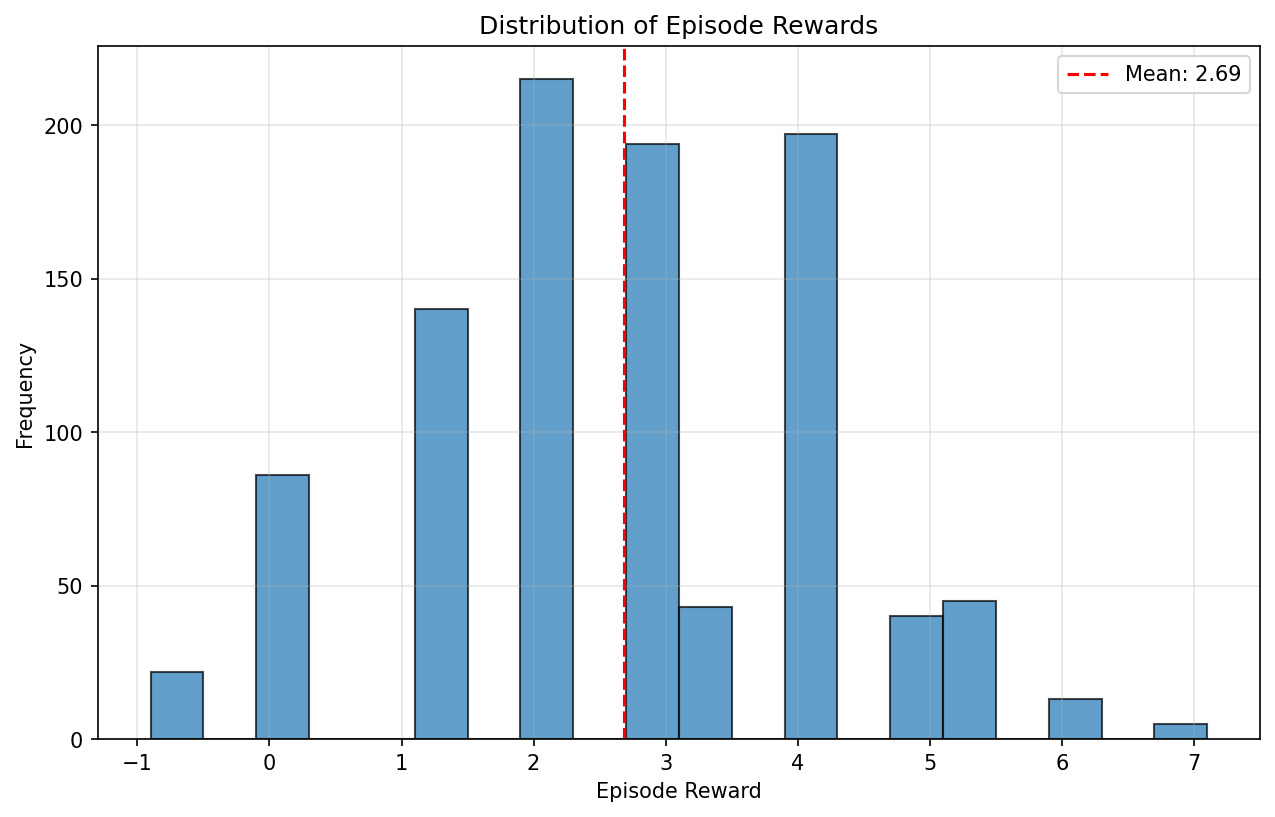
\includegraphics[width=0.75\linewidth]{images/reward_distribution_ppo_baseline.png}
    \caption{Reward distribution of PPO baseline}
    \label{fig:placeholder}
\end{figure}
\begin{figure}[H]
    \centering
    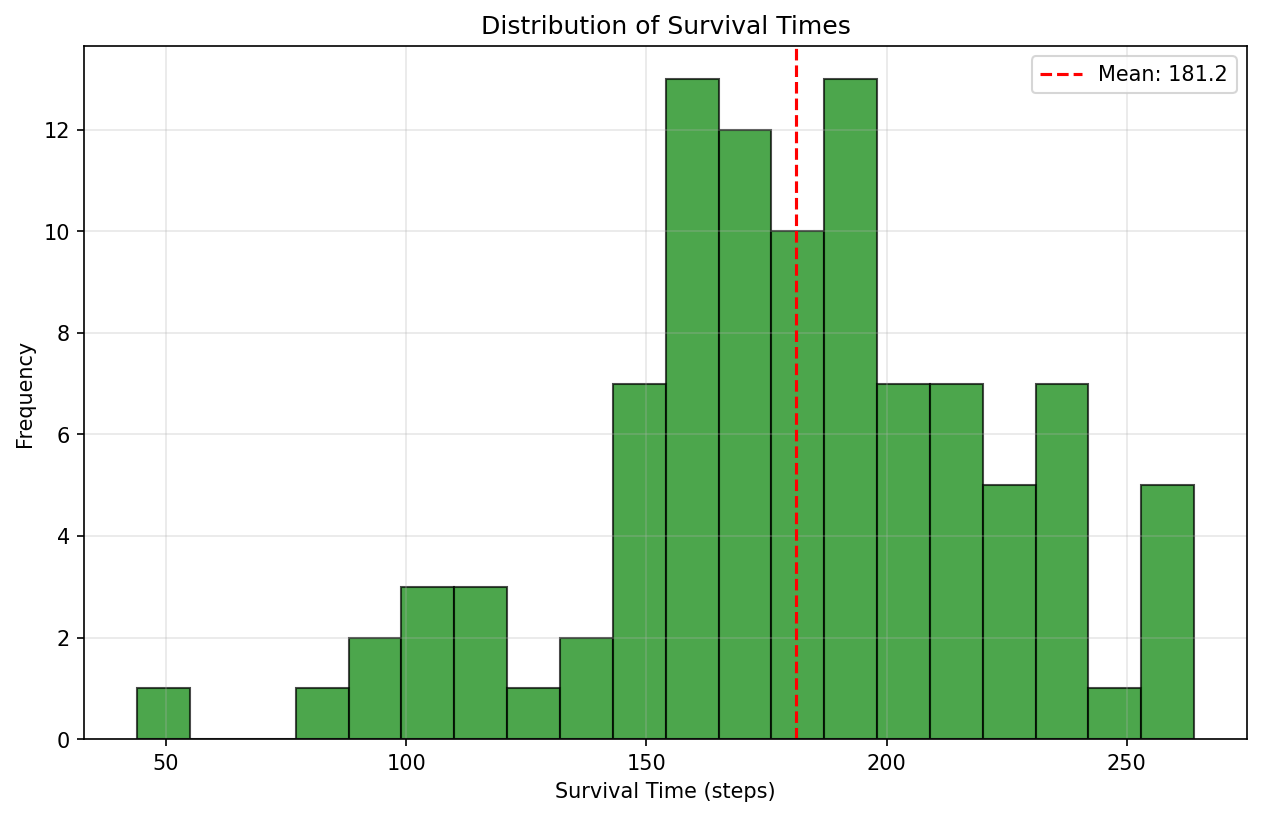
\includegraphics[width=0.75\linewidth]{images/survival_distribution_ppo_baseline.png}
    \caption{Survival distribution of PPO baseline}
    \label{fig:placeholder}
\end{figure}
\subsubsection*{Identified areas of improvement}
The following weaknesses were identified in the baseline model:
\begin{itemize}
    \item \textbf{Lack of Memory:} The agent cannot recall previous states or actions, leading to suboptimal long-term decision-making.
    \item \textbf{Limited Exploration:} Without memory or intrinsic motivation, exploration remained shallow, resulting in repetitive behavior.
\end{itemize}
\subsubsection*{Improvements and Methodology}
To address these issues, a Recurrent PPO (R-PPO) architecture was introduced. This variant augments the standard PPO with a recurrent neural network (RNN) layer, allowing the policy to maintain an internal state across time steps. This addition provides the agent with short-term memory, improving decision consistency under partial observability.

\subsection*{Improvement 1: Random Network Distillation}
\subsubsection*{Background}
Random Network Distillation (RND) is an exploration method that encourages reinforcement learning agents to explore novel states by providing intrinsic rewards based on prediction error. The method uses two neural networks: a target network that is randomly initialized and kept fixed, and a predictor network that is trained to predict the target network's outputs. The target network maps observations to feature vectors and remains frozen throughout training. The predictor network shares the same input-output architecture and is trained via gradient descent to minimize the mean squared error. The intrinsic reward is computed as the prediction error. This error is high for novel or infrequent states (where the predictor hasn't learned well) and low for frequently visited states (where the predictor has converged). \parencite{burda2018exploration}

\subsubsection*{Methodology}
\textbf{\textit{Architecture}}\\
\textit{Target Network (Fixed Random Features)} \\
The target network is a randomly initialized convolutional neural network that remains fixed throughout training. It processes $64 \times 64 \times 3$ RGB observations through three convolutional layers:
\begin{itemize}
    \item Conv1: 32 filters, $3 \times 3$ kernel, stride 2, padding 1 $\rightarrow$ output: $32 \times 32 \times 32$
    \item Conv2: 64 filters, $3 \times 3$ kernel, stride 2, padding 1 $\rightarrow$ output: $16 \times 16 \times 64$
    \item Conv3: 64 filters, $3 \times 3$ kernel, stride 1, padding 1 $\rightarrow$ output: $16 \times 16 \times 64$
    \item Flatten and fully connected layers: $16{,}384 \rightarrow 512$ features
\end{itemize}

All parameters are frozen after initialization to maintain consistent random target features.\\\\
\textit{Predictor Network (Learned Features)} \\
The predictor network shares an identical architecture with the target network but is trained to predict the target network's output. The prediction error serves as the intrinsic reward signal, where high error indicates novel states.\\\\
\textbf{\textit{Intrinsic Reward Computation}}\\
For each observed state $s_t$, the intrinsic reward is computed as:
\begin{equation}
r_{\text{intrinsic}}(s_t) = \|f_{\text{target}}(s_t) - f_{\text{predictor}}(s_t)\|^2
\end{equation}
where $f_{\text{target}}$ and $f_{\text{predictor}}$ are the outputs of the target and predictor networks respectively. The intrinsic rewards are normalized using running mean and variance statistics to maintain stable learning dynamics.\\\\
\textbf{\textit{Reward Integration}}\\
The total reward combines extrinsic (environment) and intrinsic rewards:
\begin{equation}
r_{\text{total}}(s_t) = r_{\text{extrinsic}}(s_t) + \lambda \cdot r_{\text{intrinsic}}(s_t)
\end{equation}
where $\lambda$ is the intrinsic reward coefficient (set to 1.0 by default). This is implemented via a custom Gymnasium wrapper (\texttt{RNDRewardWrapper}) that intercepts environment steps and augments rewards before they reach the PPO algorithm.\\\\
\textbf{\textit{Training Procedure}}
\begin{itemize}
    \item \textbf{RND Module Updates:} The predictor network is trained using mean squared error loss between its outputs and the fixed target network outputs. The optimizer uses Adam with learning rate $1 \times 10^{-4}$.

    \item \textbf{PPO Training:} The PPO agent is trained on the combined reward signal using standard hyperparameters and the following:
\begin{itemize}
    \item $intrinsic\_reward\_coef=1.0$
    \item $rnd\_learning\_rate=1\times10^{-4}$
\end{itemize}

\item \textbf{Evaluation Protocol:} Agent performance is evaluated every 10,000 training steps using deterministic policy rollouts over 5 episodes in a separate evaluation environment. Metrics including mean reward, standard deviation, minimum/maximum rewards, and episode lengths are logged to CSV files for analysis.
\end{itemize}
\textbf{\textit{Exploration Mechanism}}\\
The RND method encourages exploration through the following mechanism:
\begin{enumerate}
    \item Novel states produce high prediction errors, yielding high intrinsic rewards
    \item The agent is incentivized to visit these high-reward states
    \item As states become familiar, the predictor improves, reducing intrinsic rewards
    \item The agent naturally shifts focus toward extrinsic task rewards
\end{enumerate}
This approach addresses the sparse reward problem in Crafter by providing dense exploration bonuses while maintaining the original task structure.\\\\
\textbf{\textit{Implementation Details}}\\
The implementation utilizes PyTorch for neural networks and Stable Baselines3 for the PPO algorithm. The RND networks use $3 \times 3$ convolutional kernels optimized for Crafter's $64 \times 64$ observation space. Running statistics for reward normalization use Welford's online algorithm to maintain numerical stability. All experiments use seed 42 for reproducibility, with the evaluation environment seeded at 142 to ensure different but deterministic trajectories.
\subsubsection*{Results}
\begin{figure}[h]
    \centering
    \includegraphics[width=1\linewidth]{PPO Improvement 1 Evaluation Performance.png}
    \caption{PPO Improvement 1 Evaluation Performance}
    \label{fig:placeholder}
\end{figure}
\subsubsection*{Discussion}
\textbf{\textit{Differences from Standard RND Implementation}}\\
This implementation differs from the standard Random Network Distillation approach proposed by \cite{burda2018exploration} in several key aspects. The standard RND implementation uses two separate value functions---one for extrinsic returns and one for intrinsic returns---allowing different discount factors to be applied (typically $\gamma=0.99$ for intrinsic and $\gamma=0.999$ for extrinsic rewards), whereas this implementation uses a single combined value function with a uniform discount factor of 0.99. The CNN architecture has been simplified and adapted for Crafter's $64 \times 64$ observation space, using smaller $3 \times 3$ kernels throughout instead of the larger $8 \times 8$ and $4 \times 4$ kernels designed for $84 \times 84$ Atari frames, and omitting batch normalization and other regularization layers. Unlike standard RND which normalizes observations before feeding them to the RND networks and maintains separate statistics for intrinsic and extrinsic rewards, this implementation applies only basic running statistics normalization to intrinsic rewards using Welford's algorithm, with raw observations fed directly to the networks. The standard approach typically employs 128 or more parallel environments for efficient data collection and diverse training batches, updating the predictor network on mini-batches from the rollout buffer with multiple gradient steps per rollout, whereas this implementation uses a single environment instance with per-step predictor updates, resulting in slower data collection and potentially noisier gradient estimates. Additionally, standard RND implementations include explicit reward clipping to prevent extreme values, separate advantage normalization for intrinsic and extrinsic components, and curiosity-driven exploration decay schedules, none of which are present in this implementation which uses a fixed intrinsic reward coefficient. Finally, the evaluation procedure differs: standard RND evaluates with intrinsic rewards completely disabled to measure true task performance without exploration bonuses, while this implementation uses deterministic policy evaluation without explicitly disabling the RND wrapper, making the separation between exploration and exploitation performance less clear.
\subsection*{Improvement 2: Long-Short Term Memory}

\subsubsection*{Improvement 2 Implementation}
To address the baseline and improvement 1 limitations in memory and exploration, we implemented a \textbf{Recurrent Proximal Policy Optimization (Recurrent PPO)} agent. This model extends PPO by incorporating a Long Short-Term Memory (LSTM) layer, enabling the policy to retain temporal context across time steps. This memory mechanism helps the agent handle the partially observable nature of the Crafter environment, where important state information may not be visible in a single frame.
The following hyperparameters were added in addition to the previous implementations:

\begin{itemize}
    \item \textbf{Value function coefficient ($vf\_coef$):} 0.5
    \item \textbf{Maximum gradient norm ($max\_grad\_norm$):} 0.5
    \item \textbf{Reward shaping:} Enabled (\texttt{use\_reward\_shaping=True})
\end{itemize}


Additonally, slight reward shaping was employed to accelerate convergence and guide exploration towards useful sub-goals. This ensured that intermediate achievements (such as crafting tools or collecting resources) contributed meaningful gradient signals during training.
\begin{figure}[H]
    \centering
    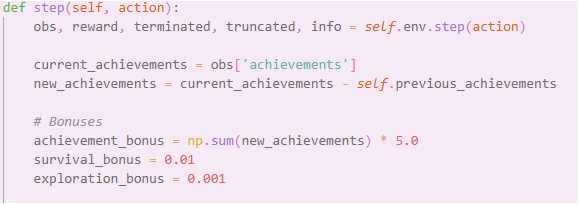
\includegraphics[width=0.5\linewidth]{images/RewardShaping.png}
    \caption{Reward Shaping implemented in RecurrentPPO agent}
\end{figure}

\subsubsection*{Observations and Performance}
The introduction of temporal recurrence through an LSTM notably improved the agent's ability to integrate information across time steps. Compared to the baseline PPO model, which achieved a mean episodic reward of approximately 3.26 (maximum 7.1), the Recurrent PPO (R-PPO) demonstrated consistent performance gains.

\subsubsection*{Qualitative Observations}

Behaviorally, the Recurrent PPO agent demonstrated:
\begin{itemize}
    \item More coherent decision sequences across time, owing to the LSTM's memory retention.
    \item Improved persistence in long-horizon tasks such as crafting and navigation.
    \item Less tendency to repeat suboptimal exploration patterns seen in the baseline agent.
\end{itemize}

In addition, reward shaping contributed to smoother early learning and faster convergence during training, as the agent received structured feedback for intermediate achievements.

\subsubsection*{Discussion}

The performance gain from incorporating temporal memory validates the hypothesis that Crafter's partial observability penalizes stateless architectures. By maintaining a hidden state, the Recurrent PPO agent effectively constructs an implicit representation of unobserved parts of the environment. This allows for more context-aware actions and ultimately leads to higher cumulative rewards. 

While the improvement is evident, the results also reveal that the agent has not fully stabilized—indicated by the wide reward range. Further tuning of learning rate, clipping threshold, and recurrent hidden size could reduce variance and enhance consistency across episodes.

The following figures show the different reward and survival distribution rates over 100 episodes:

\begin{figure}[H]
    \centering
    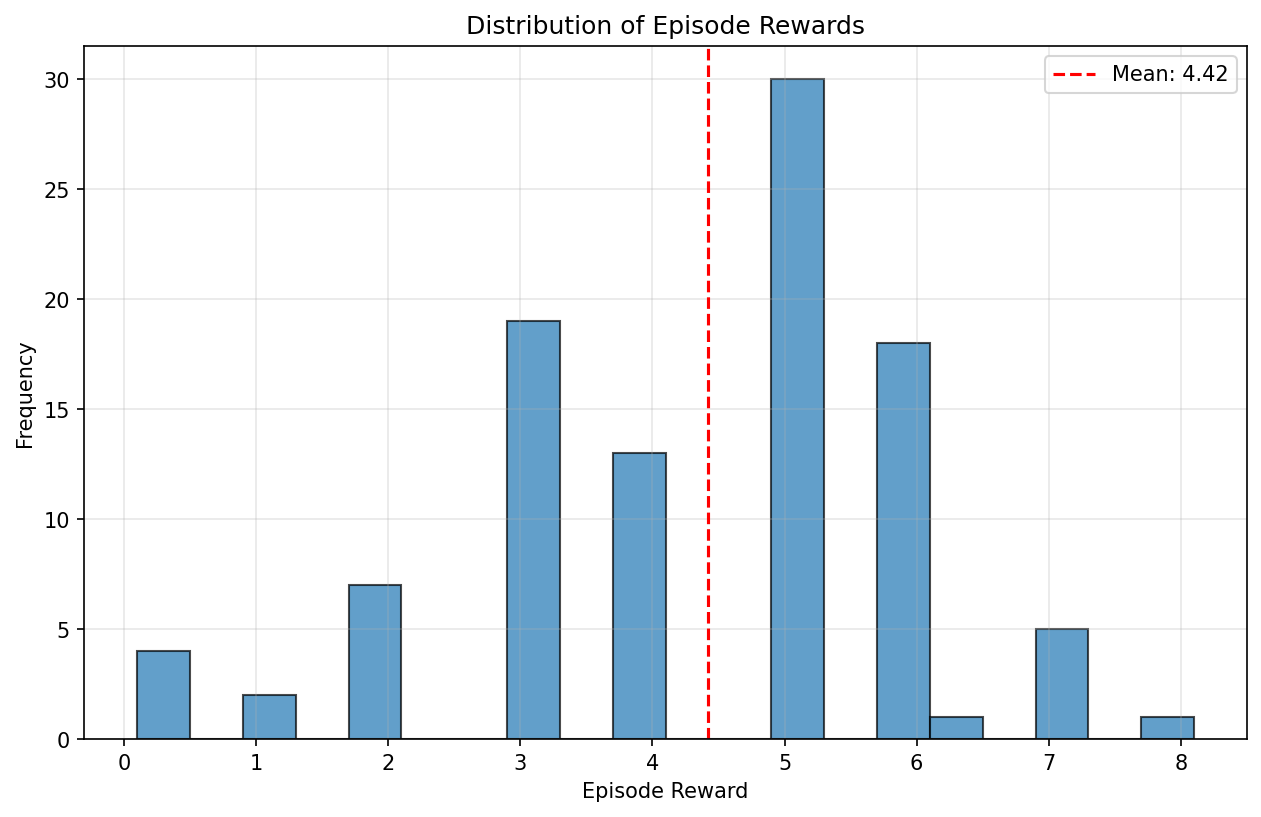
\includegraphics[width=0.75\linewidth]{images/reward_distribution_ppo_improv2.png}
    \caption{Reward distribution of PPO baseline}
    \label{fig:placeholder}
\end{figure}
\begin{figure}[H]
    \centering
    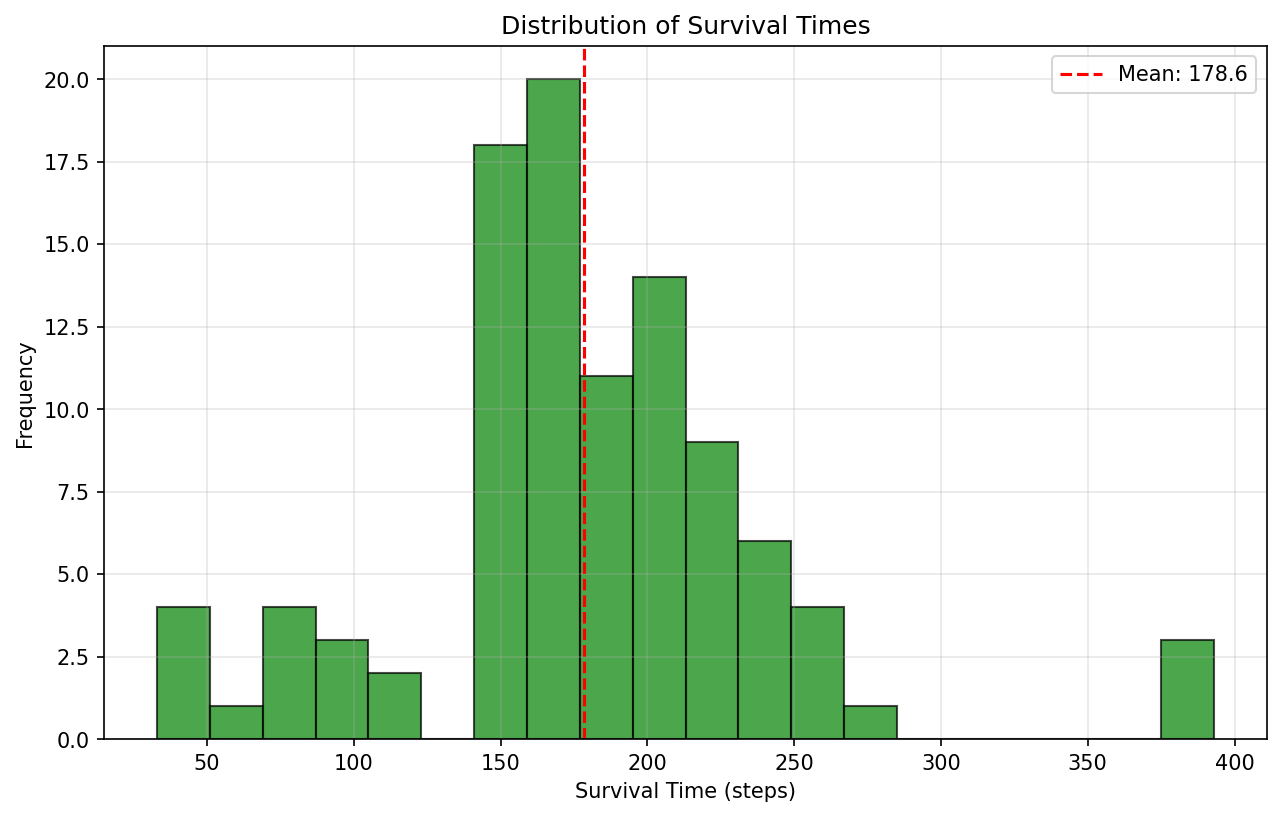
\includegraphics[width=0.75\linewidth]{images/survival_distribution_ppo_improv2.png}
    \caption{Survival distribution of PPO baseline}
    \label{fig:placeholder}
\end{figure}

An interesting observation from the experiments was that the Recurrent PPO (R-PPO) agent achieved a higher average reward (4.42) than the baseline PPO (3.26), despite exhibiting a lower overall survival rate. This contradiction can be explained by the agent's behavioral bias toward short-term, high-value actions.

The inclusion of memory through the LSTM layer allowed the agent to recall and exploit previously observed opportunities, such as nearby resources or enemies, resulting in higher reward density per timestep. However, this same decisiveness increased exposure to risk, reducing overall survival time.

Additionally, the use of reward shaping likely amplified this effect by reinforcing immediate sub-goal completion (e.g., crafting, combat) rather than conservative, long-term survival strategies. Consequently, the R-PPO learned to act more efficiently but less cautiously, prioritizing cumulative reward over lifespan duration.

This highlights a fundamental reinforcement learning trade-off between \textit{reward maximization} and \textit{survival optimization}, emphasizing that longer episodes do not necessarily equate to better task performance.

\begin{figure}[H]
    \centering
    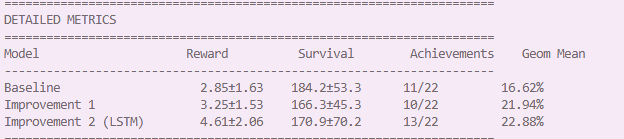
\includegraphics[width=0.75\linewidth]{images/ComparisonPPO.jpg}
    \caption{Comparison Metrics accross all PPO agents}
    \label{fig:placeholder}
\end{figure}


\end{document}
